\PassOptionsToPackage{unicode=true}{hyperref} % options for packages loaded elsewhere
\PassOptionsToPackage{hyphens}{url}
\PassOptionsToPackage{dvipsnames,svgnames*,x11names*}{xcolor}
%
\documentclass[onecolumn]{article}
\usepackage{lmodern}
\usepackage{amssymb,amsmath}
\usepackage{ifxetex,ifluatex}
\usepackage{fixltx2e} % provides \textsubscript
\ifnum 0\ifxetex 1\fi\ifluatex 1\fi=0 % if pdftex
  \usepackage[T1]{fontenc}
  \usepackage[utf8]{inputenc}
  \usepackage{textcomp} % provides euro and other symbols
\else % if luatex or xelatex
  \usepackage{unicode-math}
  \defaultfontfeatures{Ligatures=TeX,Scale=MatchLowercase}
\fi
% use upquote if available, for straight quotes in verbatim environments
\IfFileExists{upquote.sty}{\usepackage{upquote}}{}
% use microtype if available
\IfFileExists{microtype.sty}{%
\usepackage[]{microtype}
\UseMicrotypeSet[protrusion]{basicmath} % disable protrusion for tt fonts
}{}
\IfFileExists{parskip.sty}{%
\usepackage{parskip}
}{% else
\setlength{\parindent}{4pt}
\setlength{\parskip}{6pt plus 2pt minus 1pt}
}
\usepackage{xcolor}
\usepackage{hyperref}
\hypersetup{
            pdftitle={Greg Gloor},
            colorlinks=true,
            linkcolor=Maroon,
            filecolor=Maroon,
            citecolor=Blue,
            urlcolor=blue,
            breaklinks=true}
\urlstyle{same}  % don't use monospace font for urls
\usepackage[margin=2cm]{geometry}
\usepackage{graphicx,grffile}
\makeatletter
\def\maxwidth{\ifdim\Gin@nat@width>\linewidth\linewidth\else\Gin@nat@width\fi}
\def\maxheight{\ifdim\Gin@nat@height>\textheight\textheight\else\Gin@nat@height\fi}
\makeatother
% Scale images if necessary, so that they will not overflow the page
% margins by default, and it is still possible to overwrite the defaults
% using explicit options in \includegraphics[width, height, ...]{}
\setkeys{Gin}{width=\maxwidth,height=\maxheight,keepaspectratio}
\setlength{\emergencystretch}{3em}  % prevent overfull lines
\providecommand{\tightlist}{%
  \setlength{\itemsep}{0pt}\setlength{\parskip}{0pt}}
\setcounter{secnumdepth}{0}
% Redefines (sub)paragraphs to behave more like sections
\ifx\paragraph\undefined\else
\let\oldparagraph\paragraph
\renewcommand{\paragraph}[1]{\oldparagraph{#1}\mbox{}}
\fi
\ifx\subparagraph\undefined\else
\let\oldsubparagraph\subparagraph
\renewcommand{\subparagraph}[1]{\oldsubparagraph{#1}\mbox{}}
\fi

% set default figure placement to htbp
\makeatletter
\def\fps@figure{htbp}
\makeatother


\title{Greg Gloor}
\author{}
\date{\vspace{-2.5em}}

\begin{document}
\pagenumbering{gobble}
\maketitle

\vspace{-1cm}

\begin{center}
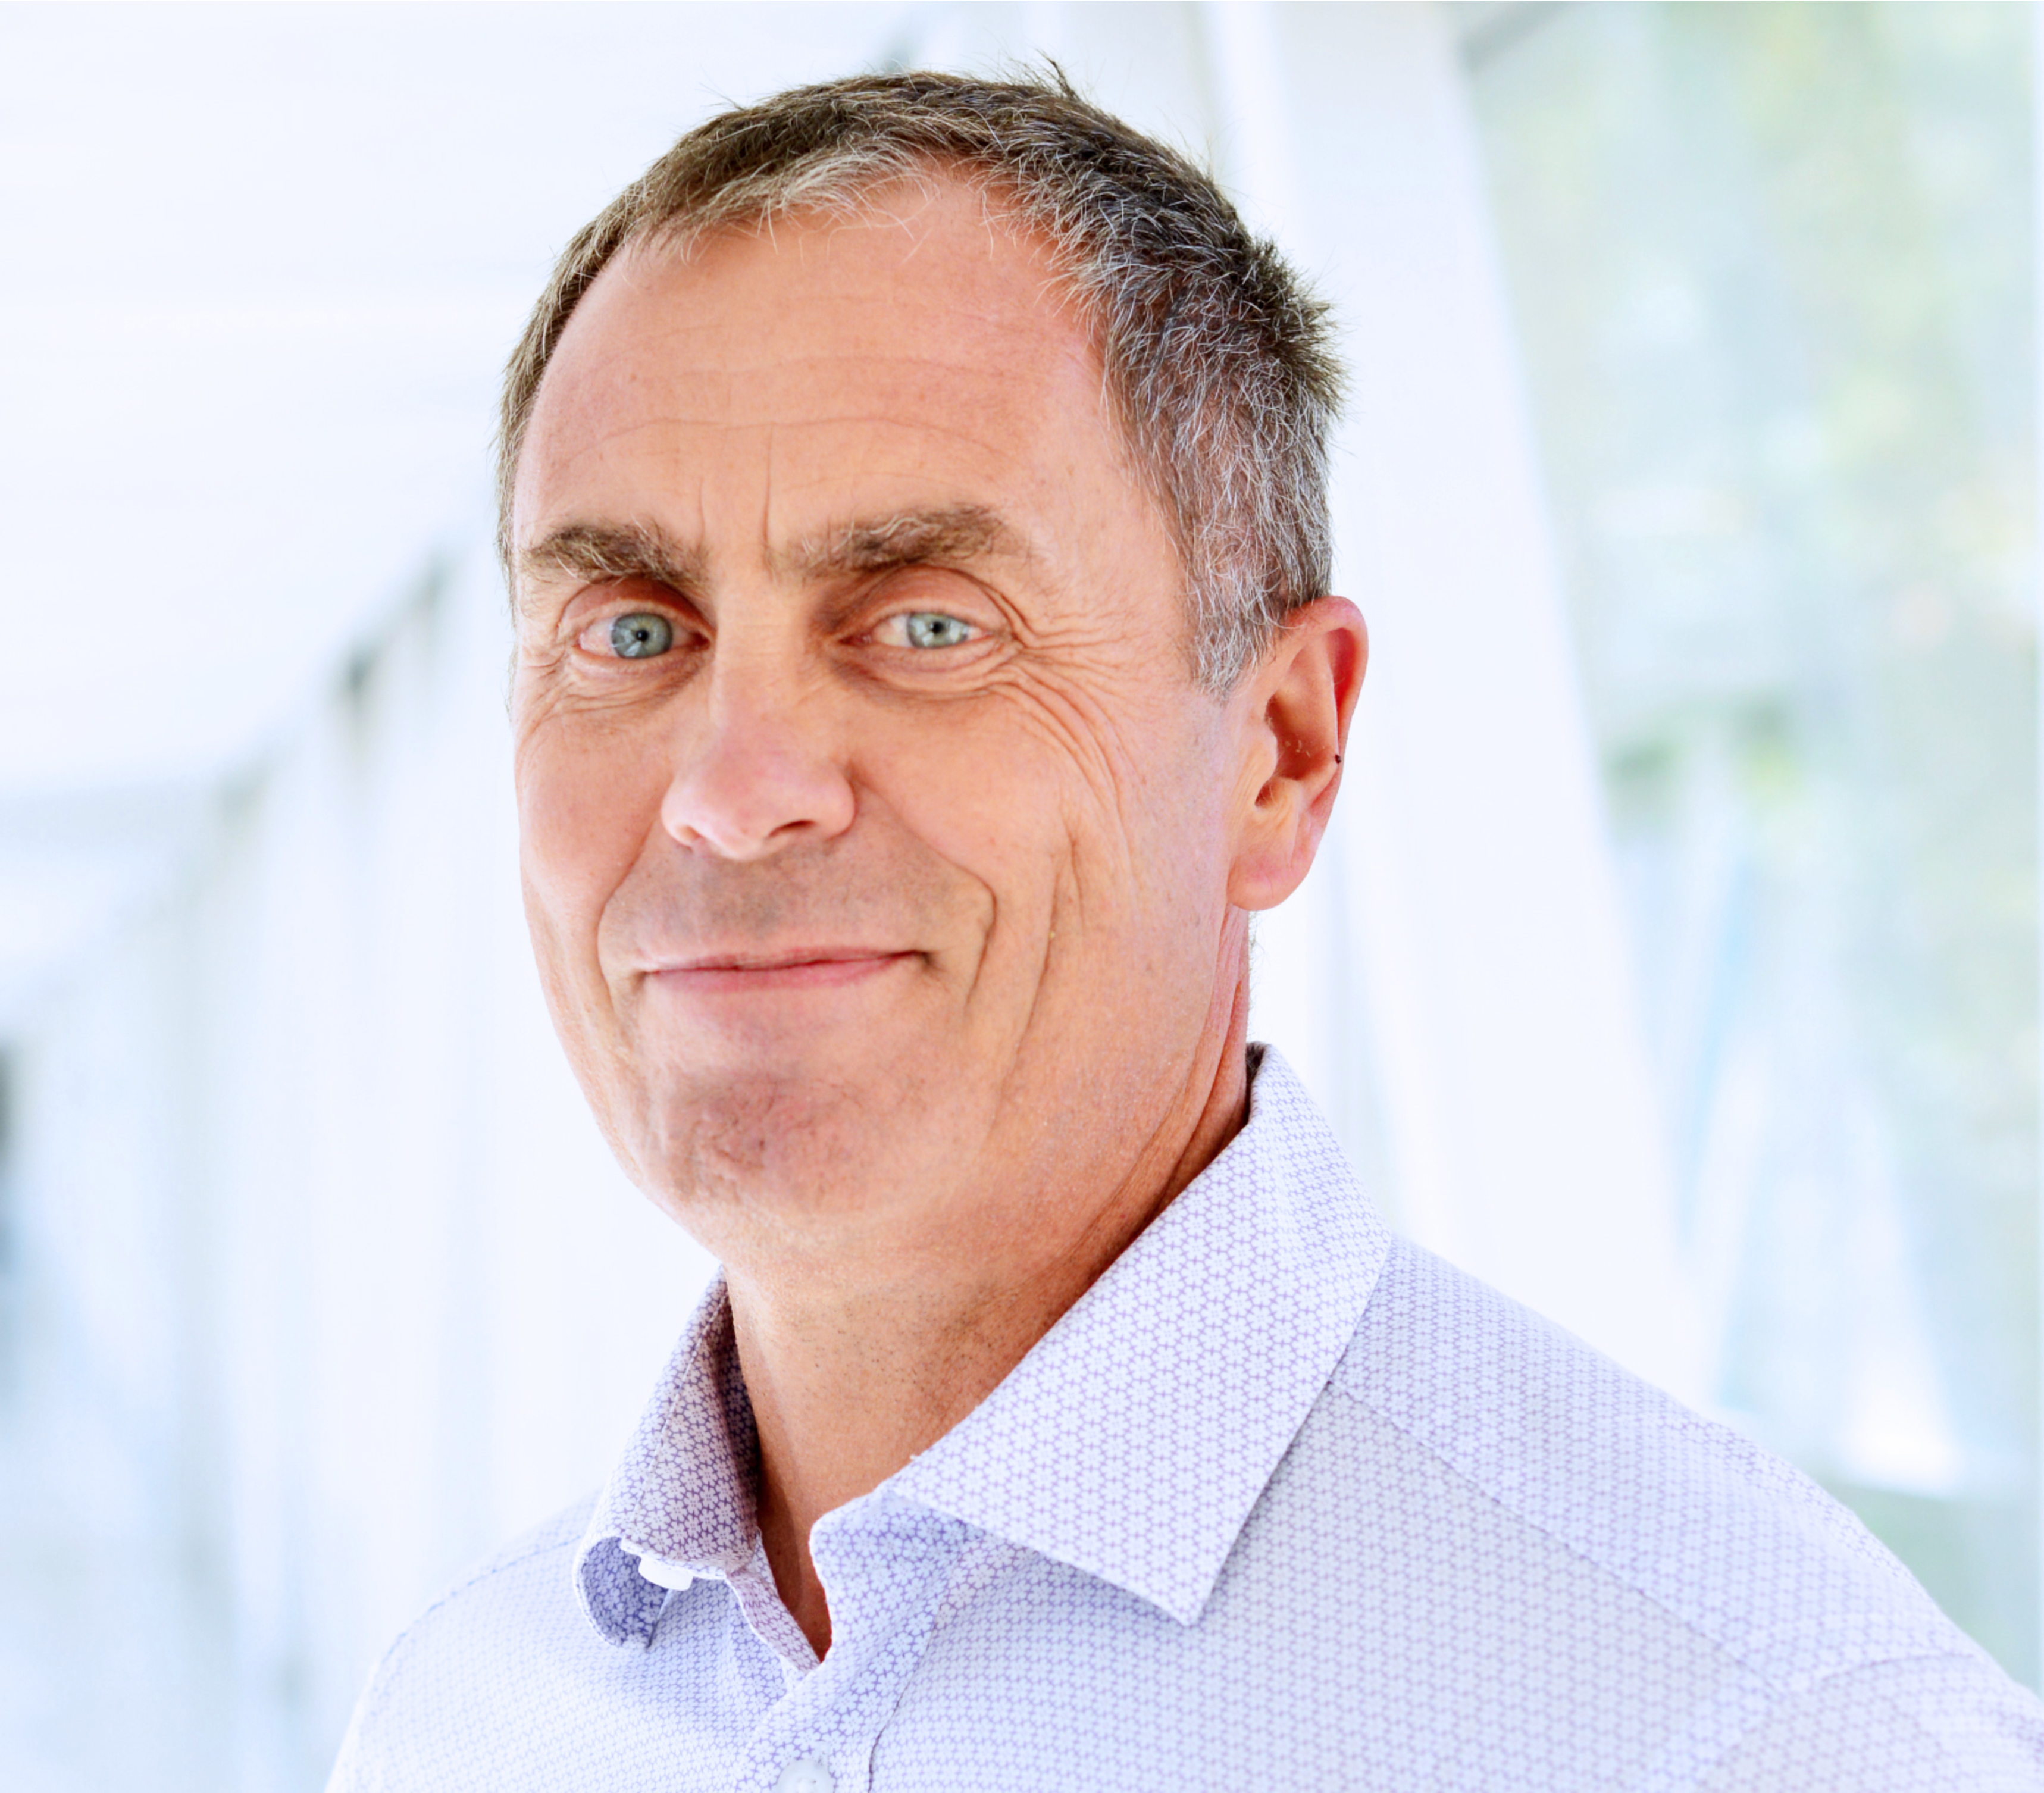
\includegraphics[width=0.45\textwidth,height=\textheight]{gg_head.pdf}
\end{center}
I am very honoured to be nominated for the position of Vice-President of
the CoDa Association. I have a PhD in Biochemistry and a very broad
research training that includes biochemistry, molecular biology,
genetics, genomics, bioinformatics and most recently data analysis. I
attended the 2014 CoDa course and found it to be invaluable because it introduced me to a wonderful
community of like-minded people. I have attended every CoDaWorks since,
making it a priority  to attend because of both the science and the
social aspects. I had the good fortune to participate in the  L'Escala meeting where the CoDa Association was formed, and to participate the first ever general meeting.

I have administrative expertise in a number of areas. I have been an
Associate or Section Editor of the journal \emph{Microbiome} since its
inception. I am Chair of the Canadian Institutes of Health Research peer
review study section on `'Genomics, Systems and Computational Biology''.
I am Professor and Chair of the Department of Biochemistry at the
University of Western Ontario. I have an open and collaborative style of
leadership and enjoy new opportunities.

I have been a consistent and vocal promoter of compositional data
analysis as a generally useful tool in biomedical research areas
that include microbiome, metagenome and transcriptome analyses of high
throughput sequencing analysis. I have travelled to four continents to
give presentations and workshops on how to apply the principles of CoDa
methods for the proper (or at least better) analysis of genomic and
transcriptomic data. I have published many case studies, methods papers
and software descriptions on how to apply CoDa methods to sequencing
data. I freely admit that I am still learning --- but that is what makes
science fun --- and I greatly appreciate the collaborations that I have
formed with members of the Association, and the help I have received from the community.

If elected, I will apply my lived experiences and work diligently on
behalf of the CoDa Association to promote the proper analysis of
biomedical data. I will be an impartial conduit for the views that members of the Association bring forward
to the Board of Directors. I will ensure
that the CoDa Association is as professionally and competently managed in
the future, as it has been in the past. I will promote the CoDa
Association and the CoDa Workshops and Courses for their valuable
contributions to scientific discourse and education.

\end{document}
